\documentclass[twoside]{book}

% Packages required by doxygen
\usepackage{fixltx2e}
\usepackage{calc}
\usepackage{doxygen}
\usepackage[export]{adjustbox} % also loads graphicx
\usepackage{graphicx}
\usepackage[utf8]{inputenc}
\usepackage{makeidx}
\usepackage{multicol}
\usepackage{multirow}
\PassOptionsToPackage{warn}{textcomp}
\usepackage{textcomp}
\usepackage[nointegrals]{wasysym}
\usepackage[table]{xcolor}

% Font selection
\usepackage[T1]{fontenc}
\usepackage[scaled=.90]{helvet}
\usepackage{courier}
\usepackage{amssymb}
\usepackage{sectsty}
\renewcommand{\familydefault}{\sfdefault}
\allsectionsfont{%
  \fontseries{bc}\selectfont%
  \color{darkgray}%
}
\renewcommand{\DoxyLabelFont}{%
  \fontseries{bc}\selectfont%
  \color{darkgray}%
}
\newcommand{\+}{\discretionary{\mbox{\scriptsize$\hookleftarrow$}}{}{}}

% Page & text layout
\usepackage{geometry}
\geometry{%
  a4paper,%
  top=2.5cm,%
  bottom=2.5cm,%
  left=2.5cm,%
  right=2.5cm%
}
\tolerance=750
\hfuzz=15pt
\hbadness=750
\setlength{\emergencystretch}{15pt}
\setlength{\parindent}{0cm}
\setlength{\parskip}{3ex plus 2ex minus 2ex}
\makeatletter
\renewcommand{\paragraph}{%
  \@startsection{paragraph}{4}{0ex}{-1.0ex}{1.0ex}{%
    \normalfont\normalsize\bfseries\SS@parafont%
  }%
}
\renewcommand{\subparagraph}{%
  \@startsection{subparagraph}{5}{0ex}{-1.0ex}{1.0ex}{%
    \normalfont\normalsize\bfseries\SS@subparafont%
  }%
}
\makeatother

% Headers & footers
\usepackage{fancyhdr}
\pagestyle{fancyplain}
\fancyhead[LE]{\fancyplain{}{\bfseries\thepage}}
\fancyhead[CE]{\fancyplain{}{}}
\fancyhead[RE]{\fancyplain{}{\bfseries\leftmark}}
\fancyhead[LO]{\fancyplain{}{\bfseries\rightmark}}
\fancyhead[CO]{\fancyplain{}{}}
\fancyhead[RO]{\fancyplain{}{\bfseries\thepage}}
\fancyfoot[LE]{\fancyplain{}{}}
\fancyfoot[CE]{\fancyplain{}{}}
\fancyfoot[RE]{\fancyplain{}{\bfseries\scriptsize Generated by Doxygen }}
\fancyfoot[LO]{\fancyplain{}{\bfseries\scriptsize Generated by Doxygen }}
\fancyfoot[CO]{\fancyplain{}{}}
\fancyfoot[RO]{\fancyplain{}{}}
\renewcommand{\footrulewidth}{0.4pt}
\renewcommand{\chaptermark}[1]{%
  \markboth{#1}{}%
}
\renewcommand{\sectionmark}[1]{%
  \markright{\thesection\ #1}%
}

% Indices & bibliography
\usepackage{natbib}
\usepackage[titles]{tocloft}
\setcounter{tocdepth}{3}
\setcounter{secnumdepth}{5}
\makeindex

% Hyperlinks (required, but should be loaded last)
\usepackage{ifpdf}
\ifpdf
  \usepackage[pdftex,pagebackref=true]{hyperref}
\else
  \usepackage[ps2pdf,pagebackref=true]{hyperref}
\fi
\hypersetup{%
  colorlinks=true,%
  linkcolor=blue,%
  citecolor=blue,%
  unicode%
}

% Custom commands
\newcommand{\clearemptydoublepage}{%
  \newpage{\pagestyle{empty}\cleardoublepage}%
}

\usepackage{caption}
\captionsetup{labelsep=space,justification=centering,font={bf},singlelinecheck=off,skip=4pt,position=top}

%===== C O N T E N T S =====

\begin{document}

% Titlepage & ToC
\hypersetup{pageanchor=false,
             bookmarksnumbered=true,
             pdfencoding=unicode
            }
\pagenumbering{roman}
\begin{titlepage}
\vspace*{7cm}
\begin{center}%
{\Large My Project }\\
\vspace*{1cm}
{\large Generated by Doxygen 1.8.11}\\
\end{center}
\end{titlepage}
\clearemptydoublepage
\tableofcontents
\clearemptydoublepage
\pagenumbering{arabic}
\hypersetup{pageanchor=true}

%--- Begin generated contents ---
\chapter{Hierarchical Index}
\section{Class Hierarchy}
This inheritance list is sorted roughly, but not completely, alphabetically\+:\begin{DoxyCompactList}
\item \contentsline{section}{Fruit}{\pageref{classFruit}}{}
\begin{DoxyCompactList}
\item \contentsline{section}{Apple}{\pageref{classApple}}{}
\item \contentsline{section}{Grape}{\pageref{classGrape}}{}
\item \contentsline{section}{Orange}{\pageref{classOrange}}{}
\end{DoxyCompactList}
\item \contentsline{section}{List}{\pageref{classList}}{}
\item \contentsline{section}{List\+:\+:Node}{\pageref{structList_1_1Node}}{}
\end{DoxyCompactList}

\chapter{Class Index}
\section{Class List}
Here are the classes, structs, unions and interfaces with brief descriptions\+:\begin{DoxyCompactList}
\item\contentsline{section}{\hyperlink{structnode}{node} }{\pageref{structnode}}{}
\item\contentsline{section}{\hyperlink{structnode1}{node1} }{\pageref{structnode1}}{}
\item\contentsline{section}{\hyperlink{structnode__info}{node\+\_\+info} }{\pageref{structnode__info}}{}
\end{DoxyCompactList}

\chapter{File Index}
\section{File List}
Here is a list of all files with brief descriptions\+:\begin{DoxyCompactList}
\item\contentsline{section}{\hyperlink{Lab1_8c}{Lab1.\+c} }{\pageref{Lab1_8c}}{}
\end{DoxyCompactList}

\chapter{Class Documentation}
\hypertarget{classCircleShape}{}\section{Circle\+Shape Class Reference}
\label{classCircleShape}\index{Circle\+Shape@{Circle\+Shape}}


Inheritance diagram for Circle\+Shape\+:
\nopagebreak
\begin{figure}[H]
\begin{center}
\leavevmode
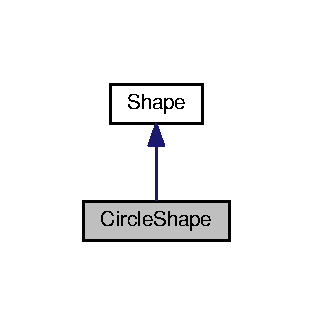
\includegraphics[width=150pt]{classCircleShape__inherit__graph}
\end{center}
\end{figure}


Collaboration diagram for Circle\+Shape\+:
\nopagebreak
\begin{figure}[H]
\begin{center}
\leavevmode
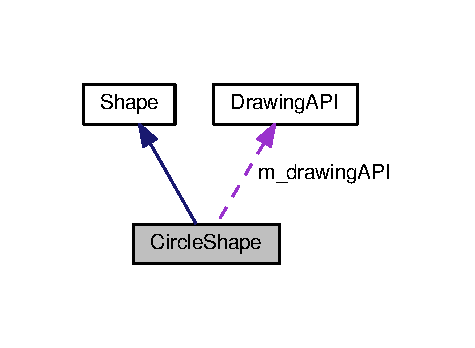
\includegraphics[width=228pt]{classCircleShape__coll__graph}
\end{center}
\end{figure}
\subsection*{Public Member Functions}
\begin{DoxyCompactItemize}
\item 
\hyperlink{classCircleShape_ad9d9792af7f2be56f6b15ffbd6629871}{Circle\+Shape} (double x, double y, double radius, \hyperlink{classDrawingAPI}{Drawing\+A\+PI} $\ast$drawing\+A\+PI)
\item 
void \hyperlink{classCircleShape_ad9f83c69677b1091ea4b2bfdb5f27c07}{draw} ()
\item 
void \hyperlink{classCircleShape_adadfd28583f61407130eee10bb33adb1}{resize\+By\+Percentage} (double pct)
\end{DoxyCompactItemize}
\subsection*{Private Attributes}
\begin{DoxyCompactItemize}
\item 
double \hyperlink{classCircleShape_a75a53e0b319fcdc17afdca4aa1e43269}{m\+\_\+x}
\item 
double \hyperlink{classCircleShape_a0889d40af7e693db62c2bb8c67182e75}{m\+\_\+y}
\item 
double \hyperlink{classCircleShape_a86f17472715fcc9dc0801876e563fbd0}{m\+\_\+radius}
\item 
\hyperlink{classDrawingAPI}{Drawing\+A\+PI} $\ast$ \hyperlink{classCircleShape_a9216b90cab92f99f48866e8af921aa5e}{m\+\_\+drawing\+A\+PI}
\end{DoxyCompactItemize}


\subsection{Constructor \& Destructor Documentation}
\index{Circle\+Shape@{Circle\+Shape}!Circle\+Shape@{Circle\+Shape}}
\index{Circle\+Shape@{Circle\+Shape}!Circle\+Shape@{Circle\+Shape}}
\subsubsection[{\texorpdfstring{Circle\+Shape(double x, double y, double radius, Drawing\+A\+P\+I $\ast$drawing\+A\+P\+I)}{CircleShape(double x, double y, double radius, DrawingAPI *drawingAPI)}}]{\setlength{\rightskip}{0pt plus 5cm}Circle\+Shape\+::\+Circle\+Shape (
\begin{DoxyParamCaption}
\item[{double}]{x, }
\item[{double}]{y, }
\item[{double}]{radius, }
\item[{{\bf Drawing\+A\+PI} $\ast$}]{drawing\+A\+PI}
\end{DoxyParamCaption}
)\hspace{0.3cm}{\ttfamily [inline]}}\hypertarget{classCircleShape_ad9d9792af7f2be56f6b15ffbd6629871}{}\label{classCircleShape_ad9d9792af7f2be56f6b15ffbd6629871}

\begin{DoxyCode}
39                                                                          :
40        \hyperlink{classCircleShape_a75a53e0b319fcdc17afdca4aa1e43269}{m\_x}(x), \hyperlink{classCircleShape_a0889d40af7e693db62c2bb8c67182e75}{m\_y}(y), \hyperlink{classCircleShape_a86f17472715fcc9dc0801876e563fbd0}{m\_radius}(radius), \hyperlink{classCircleShape_a9216b90cab92f99f48866e8af921aa5e}{m\_drawingAPI}(drawingAPI)
41    \{\}
\end{DoxyCode}


\subsection{Member Function Documentation}
\index{Circle\+Shape@{Circle\+Shape}!draw@{draw}}
\index{draw@{draw}!Circle\+Shape@{Circle\+Shape}}
\subsubsection[{\texorpdfstring{draw()}{draw()}}]{\setlength{\rightskip}{0pt plus 5cm}void Circle\+Shape\+::draw (
\begin{DoxyParamCaption}
{}
\end{DoxyParamCaption}
)\hspace{0.3cm}{\ttfamily [inline]}, {\ttfamily [virtual]}}\hypertarget{classCircleShape_ad9f83c69677b1091ea4b2bfdb5f27c07}{}\label{classCircleShape_ad9f83c69677b1091ea4b2bfdb5f27c07}


Implements \hyperlink{classShape_afacc5aad8e37308c3ce8fef768199b05}{Shape}.


\begin{DoxyCode}
42                \{
43       \hyperlink{classCircleShape_a9216b90cab92f99f48866e8af921aa5e}{m\_drawingAPI}->\hyperlink{classDrawingAPI_a7a5b900cc78619bfe10b6555608f871d}{drawCircle}(\hyperlink{classCircleShape_a75a53e0b319fcdc17afdca4aa1e43269}{m\_x}, \hyperlink{classCircleShape_a0889d40af7e693db62c2bb8c67182e75}{m\_y}, \hyperlink{classCircleShape_a86f17472715fcc9dc0801876e563fbd0}{m\_radius});
44    \}
\end{DoxyCode}
\index{Circle\+Shape@{Circle\+Shape}!resize\+By\+Percentage@{resize\+By\+Percentage}}
\index{resize\+By\+Percentage@{resize\+By\+Percentage}!Circle\+Shape@{Circle\+Shape}}
\subsubsection[{\texorpdfstring{resize\+By\+Percentage(double pct)}{resizeByPercentage(double pct)}}]{\setlength{\rightskip}{0pt plus 5cm}void Circle\+Shape\+::resize\+By\+Percentage (
\begin{DoxyParamCaption}
\item[{double}]{pct}
\end{DoxyParamCaption}
)\hspace{0.3cm}{\ttfamily [inline]}, {\ttfamily [virtual]}}\hypertarget{classCircleShape_adadfd28583f61407130eee10bb33adb1}{}\label{classCircleShape_adadfd28583f61407130eee10bb33adb1}


Implements \hyperlink{classShape_a892f1d0e57b41828f717662d3628c650}{Shape}.


\begin{DoxyCode}
45                                        \{
46       \hyperlink{classCircleShape_a86f17472715fcc9dc0801876e563fbd0}{m\_radius} *= pct;
47    \}
\end{DoxyCode}


\subsection{Member Data Documentation}
\index{Circle\+Shape@{Circle\+Shape}!m\+\_\+drawing\+A\+PI@{m\+\_\+drawing\+A\+PI}}
\index{m\+\_\+drawing\+A\+PI@{m\+\_\+drawing\+A\+PI}!Circle\+Shape@{Circle\+Shape}}
\subsubsection[{\texorpdfstring{m\+\_\+drawing\+A\+PI}{m_drawingAPI}}]{\setlength{\rightskip}{0pt plus 5cm}{\bf Drawing\+A\+PI}$\ast$ Circle\+Shape\+::m\+\_\+drawing\+A\+PI\hspace{0.3cm}{\ttfamily [private]}}\hypertarget{classCircleShape_a9216b90cab92f99f48866e8af921aa5e}{}\label{classCircleShape_a9216b90cab92f99f48866e8af921aa5e}
\index{Circle\+Shape@{Circle\+Shape}!m\+\_\+radius@{m\+\_\+radius}}
\index{m\+\_\+radius@{m\+\_\+radius}!Circle\+Shape@{Circle\+Shape}}
\subsubsection[{\texorpdfstring{m\+\_\+radius}{m_radius}}]{\setlength{\rightskip}{0pt plus 5cm}double Circle\+Shape\+::m\+\_\+radius\hspace{0.3cm}{\ttfamily [private]}}\hypertarget{classCircleShape_a86f17472715fcc9dc0801876e563fbd0}{}\label{classCircleShape_a86f17472715fcc9dc0801876e563fbd0}
\index{Circle\+Shape@{Circle\+Shape}!m\+\_\+x@{m\+\_\+x}}
\index{m\+\_\+x@{m\+\_\+x}!Circle\+Shape@{Circle\+Shape}}
\subsubsection[{\texorpdfstring{m\+\_\+x}{m_x}}]{\setlength{\rightskip}{0pt plus 5cm}double Circle\+Shape\+::m\+\_\+x\hspace{0.3cm}{\ttfamily [private]}}\hypertarget{classCircleShape_a75a53e0b319fcdc17afdca4aa1e43269}{}\label{classCircleShape_a75a53e0b319fcdc17afdca4aa1e43269}
\index{Circle\+Shape@{Circle\+Shape}!m\+\_\+y@{m\+\_\+y}}
\index{m\+\_\+y@{m\+\_\+y}!Circle\+Shape@{Circle\+Shape}}
\subsubsection[{\texorpdfstring{m\+\_\+y}{m_y}}]{\setlength{\rightskip}{0pt plus 5cm}double Circle\+Shape\+::m\+\_\+y\hspace{0.3cm}{\ttfamily [private]}}\hypertarget{classCircleShape_a0889d40af7e693db62c2bb8c67182e75}{}\label{classCircleShape_a0889d40af7e693db62c2bb8c67182e75}


The documentation for this class was generated from the following file\+:\begin{DoxyCompactItemize}
\item 
\hyperlink{Bridge_8cpp}{Bridge.\+cpp}\end{DoxyCompactItemize}

\hypertarget{classDrawingAPI}{}\section{Drawing\+A\+PI Class Reference}
\label{classDrawingAPI}\index{Drawing\+A\+PI@{Drawing\+A\+PI}}


Inheritance diagram for Drawing\+A\+PI\+:
\nopagebreak
\begin{figure}[H]
\begin{center}
\leavevmode
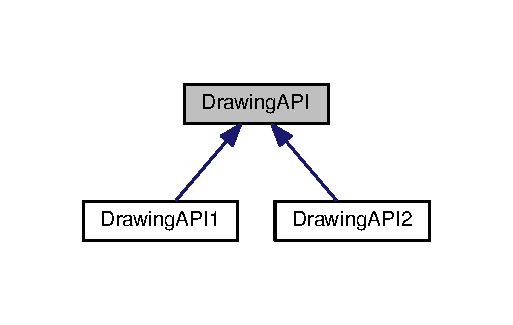
\includegraphics[width=246pt]{classDrawingAPI__inherit__graph}
\end{center}
\end{figure}
\subsection*{Public Member Functions}
\begin{DoxyCompactItemize}
\item 
virtual void \hyperlink{classDrawingAPI_a7a5b900cc78619bfe10b6555608f871d}{draw\+Circle} (double x, double y, double radius)=0
\item 
virtual \hyperlink{classDrawingAPI_a1a8ba83e77bef8ce4f91f673bc8f91df}{$\sim$\+Drawing\+A\+PI} ()
\end{DoxyCompactItemize}


\subsection{Constructor \& Destructor Documentation}
\index{Drawing\+A\+PI@{Drawing\+A\+PI}!````~Drawing\+A\+PI@{$\sim$\+Drawing\+A\+PI}}
\index{````~Drawing\+A\+PI@{$\sim$\+Drawing\+A\+PI}!Drawing\+A\+PI@{Drawing\+A\+PI}}
\subsubsection[{\texorpdfstring{$\sim$\+Drawing\+A\+P\+I()}{~DrawingAPI()}}]{\setlength{\rightskip}{0pt plus 5cm}virtual Drawing\+A\+P\+I\+::$\sim$\+Drawing\+A\+PI (
\begin{DoxyParamCaption}
{}
\end{DoxyParamCaption}
)\hspace{0.3cm}{\ttfamily [inline]}, {\ttfamily [virtual]}}\hypertarget{classDrawingAPI_a1a8ba83e77bef8ce4f91f673bc8f91df}{}\label{classDrawingAPI_a1a8ba83e77bef8ce4f91f673bc8f91df}

\begin{DoxyCode}
9 \{\}
\end{DoxyCode}


\subsection{Member Function Documentation}
\index{Drawing\+A\+PI@{Drawing\+A\+PI}!draw\+Circle@{draw\+Circle}}
\index{draw\+Circle@{draw\+Circle}!Drawing\+A\+PI@{Drawing\+A\+PI}}
\subsubsection[{\texorpdfstring{draw\+Circle(double x, double y, double radius)=0}{drawCircle(double x, double y, double radius)=0}}]{\setlength{\rightskip}{0pt plus 5cm}virtual void Drawing\+A\+P\+I\+::draw\+Circle (
\begin{DoxyParamCaption}
\item[{double}]{x, }
\item[{double}]{y, }
\item[{double}]{radius}
\end{DoxyParamCaption}
)\hspace{0.3cm}{\ttfamily [pure virtual]}}\hypertarget{classDrawingAPI_a7a5b900cc78619bfe10b6555608f871d}{}\label{classDrawingAPI_a7a5b900cc78619bfe10b6555608f871d}


Implemented in \hyperlink{classDrawingAPI2_a1a5df894023a891c2fc53ca76197bb01}{Drawing\+A\+P\+I2}, and \hyperlink{classDrawingAPI1_a53f3e670724c097445f342824ddf434e}{Drawing\+A\+P\+I1}.



The documentation for this class was generated from the following file\+:\begin{DoxyCompactItemize}
\item 
\hyperlink{Bridge_8cpp}{Bridge.\+cpp}\end{DoxyCompactItemize}

\hypertarget{classDrawingAPI1}{}\section{Drawing\+A\+P\+I1 Class Reference}
\label{classDrawingAPI1}\index{Drawing\+A\+P\+I1@{Drawing\+A\+P\+I1}}


Inheritance diagram for Drawing\+A\+P\+I1\+:
\nopagebreak
\begin{figure}[H]
\begin{center}
\leavevmode
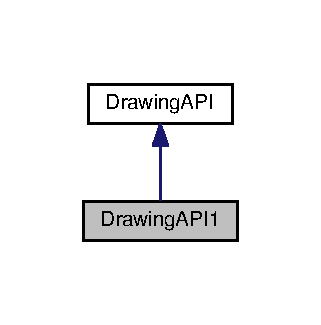
\includegraphics[width=154pt]{classDrawingAPI1__inherit__graph}
\end{center}
\end{figure}


Collaboration diagram for Drawing\+A\+P\+I1\+:
\nopagebreak
\begin{figure}[H]
\begin{center}
\leavevmode
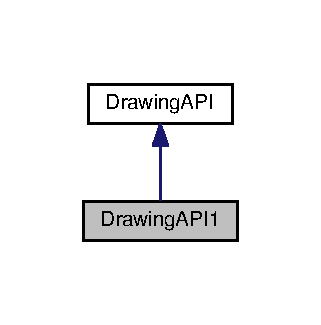
\includegraphics[width=154pt]{classDrawingAPI1__coll__graph}
\end{center}
\end{figure}
\subsection*{Public Member Functions}
\begin{DoxyCompactItemize}
\item 
void \hyperlink{classDrawingAPI1_a53f3e670724c097445f342824ddf434e}{draw\+Circle} (double x, double y, double radius)
\end{DoxyCompactItemize}


\subsection{Member Function Documentation}
\index{Drawing\+A\+P\+I1@{Drawing\+A\+P\+I1}!draw\+Circle@{draw\+Circle}}
\index{draw\+Circle@{draw\+Circle}!Drawing\+A\+P\+I1@{Drawing\+A\+P\+I1}}
\subsubsection[{\texorpdfstring{draw\+Circle(double x, double y, double radius)}{drawCircle(double x, double y, double radius)}}]{\setlength{\rightskip}{0pt plus 5cm}void Drawing\+A\+P\+I1\+::draw\+Circle (
\begin{DoxyParamCaption}
\item[{double}]{x, }
\item[{double}]{y, }
\item[{double}]{radius}
\end{DoxyParamCaption}
)\hspace{0.3cm}{\ttfamily [inline]}, {\ttfamily [virtual]}}\hypertarget{classDrawingAPI1_a53f3e670724c097445f342824ddf434e}{}\label{classDrawingAPI1_a53f3e670724c097445f342824ddf434e}


Implements \hyperlink{classDrawingAPI_a7a5b900cc78619bfe10b6555608f871d}{Drawing\+A\+PI}.


\begin{DoxyCode}
15                                                       \{
16       cout << \textcolor{stringliteral}{"API1.circle at "} << x << \textcolor{charliteral}{':'} << y << \textcolor{charliteral}{' '} << radius << endl;
17    \}
\end{DoxyCode}


The documentation for this class was generated from the following file\+:\begin{DoxyCompactItemize}
\item 
\hyperlink{Bridge_8cpp}{Bridge.\+cpp}\end{DoxyCompactItemize}

\hypertarget{classDrawingAPI2}{}\section{Drawing\+A\+P\+I2 Class Reference}
\label{classDrawingAPI2}\index{Drawing\+A\+P\+I2@{Drawing\+A\+P\+I2}}


Inheritance diagram for Drawing\+A\+P\+I2\+:
\nopagebreak
\begin{figure}[H]
\begin{center}
\leavevmode
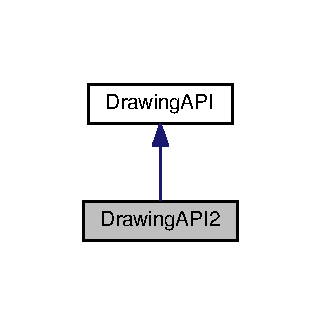
\includegraphics[width=154pt]{classDrawingAPI2__inherit__graph}
\end{center}
\end{figure}


Collaboration diagram for Drawing\+A\+P\+I2\+:
\nopagebreak
\begin{figure}[H]
\begin{center}
\leavevmode
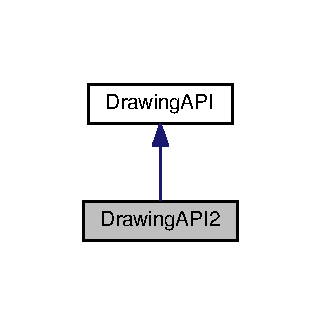
\includegraphics[width=154pt]{classDrawingAPI2__coll__graph}
\end{center}
\end{figure}
\subsection*{Public Member Functions}
\begin{DoxyCompactItemize}
\item 
void \hyperlink{classDrawingAPI2_a1a5df894023a891c2fc53ca76197bb01}{draw\+Circle} (double x, double y, double radius)
\end{DoxyCompactItemize}


\subsection{Member Function Documentation}
\index{Drawing\+A\+P\+I2@{Drawing\+A\+P\+I2}!draw\+Circle@{draw\+Circle}}
\index{draw\+Circle@{draw\+Circle}!Drawing\+A\+P\+I2@{Drawing\+A\+P\+I2}}
\subsubsection[{\texorpdfstring{draw\+Circle(double x, double y, double radius)}{drawCircle(double x, double y, double radius)}}]{\setlength{\rightskip}{0pt plus 5cm}void Drawing\+A\+P\+I2\+::draw\+Circle (
\begin{DoxyParamCaption}
\item[{double}]{x, }
\item[{double}]{y, }
\item[{double}]{radius}
\end{DoxyParamCaption}
)\hspace{0.3cm}{\ttfamily [inline]}, {\ttfamily [virtual]}}\hypertarget{classDrawingAPI2_a1a5df894023a891c2fc53ca76197bb01}{}\label{classDrawingAPI2_a1a5df894023a891c2fc53ca76197bb01}


Implements \hyperlink{classDrawingAPI_a7a5b900cc78619bfe10b6555608f871d}{Drawing\+A\+PI}.


\begin{DoxyCode}
23                                                       \{
24       cout << \textcolor{stringliteral}{"API2.circle at "} << x << \textcolor{charliteral}{':'} << y << \textcolor{charliteral}{' '} <<  radius << endl;
25    \}
\end{DoxyCode}


The documentation for this class was generated from the following file\+:\begin{DoxyCompactItemize}
\item 
\hyperlink{Bridge_8cpp}{Bridge.\+cpp}\end{DoxyCompactItemize}

\hypertarget{classShape}{}\section{Shape Class Reference}
\label{classShape}\index{Shape@{Shape}}


Inheritance diagram for Shape\+:
\nopagebreak
\begin{figure}[H]
\begin{center}
\leavevmode
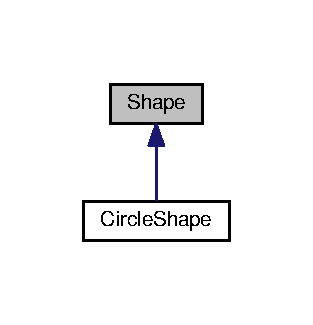
\includegraphics[width=150pt]{classShape__inherit__graph}
\end{center}
\end{figure}
\subsection*{Public Member Functions}
\begin{DoxyCompactItemize}
\item 
virtual \hyperlink{classShape_ac3b9fc48965274893f25b18aa14ba665}{$\sim$\+Shape} ()
\item 
virtual void \hyperlink{classShape_afacc5aad8e37308c3ce8fef768199b05}{draw} ()=0
\item 
virtual void \hyperlink{classShape_a892f1d0e57b41828f717662d3628c650}{resize\+By\+Percentage} (double pct)=0
\end{DoxyCompactItemize}


\subsection{Constructor \& Destructor Documentation}
\index{Shape@{Shape}!````~Shape@{$\sim$\+Shape}}
\index{````~Shape@{$\sim$\+Shape}!Shape@{Shape}}
\subsubsection[{\texorpdfstring{$\sim$\+Shape()}{~Shape()}}]{\setlength{\rightskip}{0pt plus 5cm}virtual Shape\+::$\sim$\+Shape (
\begin{DoxyParamCaption}
{}
\end{DoxyParamCaption}
)\hspace{0.3cm}{\ttfamily [inline]}, {\ttfamily [virtual]}}\hypertarget{classShape_ac3b9fc48965274893f25b18aa14ba665}{}\label{classShape_ac3b9fc48965274893f25b18aa14ba665}

\begin{DoxyCode}
31 \{\}
\end{DoxyCode}


\subsection{Member Function Documentation}
\index{Shape@{Shape}!draw@{draw}}
\index{draw@{draw}!Shape@{Shape}}
\subsubsection[{\texorpdfstring{draw()=0}{draw()=0}}]{\setlength{\rightskip}{0pt plus 5cm}virtual void Shape\+::draw (
\begin{DoxyParamCaption}
{}
\end{DoxyParamCaption}
)\hspace{0.3cm}{\ttfamily [pure virtual]}}\hypertarget{classShape_afacc5aad8e37308c3ce8fef768199b05}{}\label{classShape_afacc5aad8e37308c3ce8fef768199b05}


Implemented in \hyperlink{classCircleShape_ad9f83c69677b1091ea4b2bfdb5f27c07}{Circle\+Shape}.

\index{Shape@{Shape}!resize\+By\+Percentage@{resize\+By\+Percentage}}
\index{resize\+By\+Percentage@{resize\+By\+Percentage}!Shape@{Shape}}
\subsubsection[{\texorpdfstring{resize\+By\+Percentage(double pct)=0}{resizeByPercentage(double pct)=0}}]{\setlength{\rightskip}{0pt plus 5cm}virtual void Shape\+::resize\+By\+Percentage (
\begin{DoxyParamCaption}
\item[{double}]{pct}
\end{DoxyParamCaption}
)\hspace{0.3cm}{\ttfamily [pure virtual]}}\hypertarget{classShape_a892f1d0e57b41828f717662d3628c650}{}\label{classShape_a892f1d0e57b41828f717662d3628c650}


Implemented in \hyperlink{classCircleShape_adadfd28583f61407130eee10bb33adb1}{Circle\+Shape}.



The documentation for this class was generated from the following file\+:\begin{DoxyCompactItemize}
\item 
\hyperlink{Bridge_8cpp}{Bridge.\+cpp}\end{DoxyCompactItemize}

\chapter{File Documentation}
\hypertarget{Bridge_8cpp}{}\section{Bridge.\+cpp File Reference}
\label{Bridge_8cpp}\index{Bridge.\+cpp@{Bridge.\+cpp}}
{\ttfamily \#include $<$iostream$>$}\\*
Include dependency graph for Bridge.\+cpp\+:
\nopagebreak
\begin{figure}[H]
\begin{center}
\leavevmode
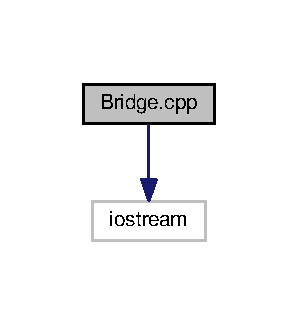
\includegraphics[width=143pt]{Bridge_8cpp__incl}
\end{center}
\end{figure}
\subsection*{Classes}
\begin{DoxyCompactItemize}
\item 
class \hyperlink{classDrawingAPI}{Drawing\+A\+PI}
\item 
class \hyperlink{classDrawingAPI1}{Drawing\+A\+P\+I1}
\item 
class \hyperlink{classDrawingAPI2}{Drawing\+A\+P\+I2}
\item 
class \hyperlink{classShape}{Shape}
\item 
class \hyperlink{classCircleShape}{Circle\+Shape}
\end{DoxyCompactItemize}
\subsection*{Functions}
\begin{DoxyCompactItemize}
\item 
int \hyperlink{Bridge_8cpp_a840291bc02cba5474a4cb46a9b9566fe}{main} (void)
\end{DoxyCompactItemize}


\subsection{Function Documentation}
\index{Bridge.\+cpp@{Bridge.\+cpp}!main@{main}}
\index{main@{main}!Bridge.\+cpp@{Bridge.\+cpp}}
\subsubsection[{\texorpdfstring{main(void)}{main(void)}}]{\setlength{\rightskip}{0pt plus 5cm}int main (
\begin{DoxyParamCaption}
\item[{void}]{}
\end{DoxyParamCaption}
)}\hypertarget{Bridge_8cpp_a840291bc02cba5474a4cb46a9b9566fe}{}\label{Bridge_8cpp_a840291bc02cba5474a4cb46a9b9566fe}

\begin{DoxyCode}
53                \{
54    \hyperlink{classCircleShape}{CircleShape} circle1(1,2,3,\textcolor{keyword}{new} \hyperlink{classDrawingAPI1}{DrawingAPI1}());
55    \hyperlink{classCircleShape}{CircleShape} circle2(5,7,11,\textcolor{keyword}{new} \hyperlink{classDrawingAPI2}{DrawingAPI2}());
56    circle1.resizeByPercentage(2.5);
57    circle2.resizeByPercentage(2.5);
58    circle1.draw();
59    circle2.draw();
60    \textcolor{keywordflow}{return} 0;
61 \}\end{DoxyCode}


Here is the call graph for this function\+:
\nopagebreak
\begin{figure}[H]
\begin{center}
\leavevmode
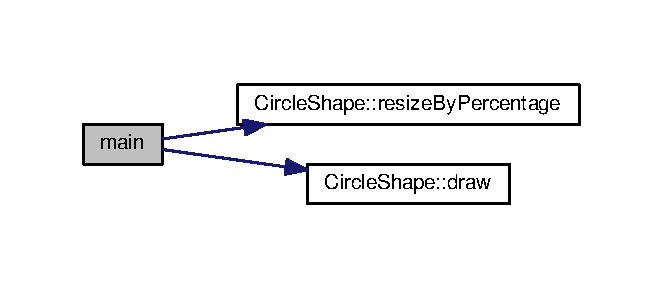
\includegraphics[width=318pt]{Bridge_8cpp_a840291bc02cba5474a4cb46a9b9566fe_cgraph}
\end{center}
\end{figure}



%--- End generated contents ---

% Index
\backmatter
\newpage
\phantomsection
\clearemptydoublepage
\addcontentsline{toc}{chapter}{Index}
\printindex

\end{document}
